\begin{appendices}

\chapter{Network Architectures} \label{appendix:network_architectures}

\begin{figure}[!tbp]
	\centering
    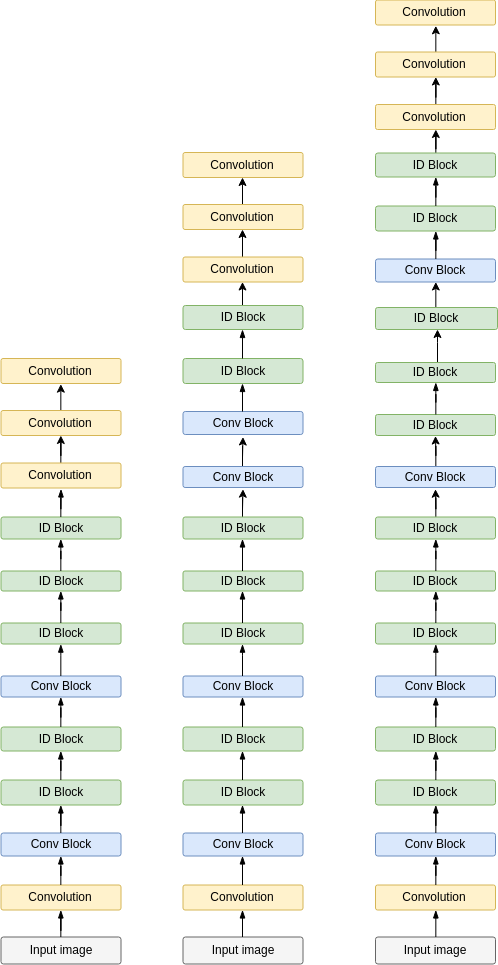
\includegraphics[width=0.7\linewidth]{network_architecture_comparison}
    \caption{The different architectures used in this work. Architectures 1 and 3 use the leftmost structure with a total of 23 convolutional layers. We constructed architecture 2 using the layout in the middle with 35 layers. Architectures 4, 5 and 6 use the 50 layers structured as shown on the right, although architectures 4 and 6 employ dropout layers with different frequencies after each block and omit the batchnormalization layers. We omitted the batchnormalization layers in the other to structures for displaying purposes.}
    \label{fig:network_architecture_comparison}
\end{figure} 

\chapter{Experiments}

\begin{figure}[!tbp]
	\centering
	\begin{subfigure}[t]{0.48\textwidth}
			\begin{tikzpicture}
  				\begin{axis}[cycle list name=tb, 
                 grid=both,
                 grid style={solid,gray!30!white},
                 axis lines=middle,
    			 xmin = 0,
    			 xmax = 100,
    			 ymin = 0,
    			 ymax = 3,
                 xlabel={step},
                 ylabel={value},
                 x label style={at={(axis description cs:0.5,-0.1)},anchor=north},
                 y label style={at={(axis description cs:-0.1,.5)},rotate=90,anchor=south},]
      			\addplot[smooth,tb_color_1] table [x=Step, y=Value, col sep=comma] {experiments/model1/exp1_adam_l1/train_loss.csv};
      			\addplot[smooth,tb_color_2] table [x=Step, y=Value, col sep=comma] {experiments/model1/exp1_adam_l2/train_loss.csv};
      			\addlegendentry{L1}
				\addlegendentry{L2}
    			\end{axis}
			\end{tikzpicture}
		\caption{Training losses.}
	\end{subfigure}
	\hfill
	\begin{subfigure}[t]{0.48\textwidth}
			\begin{tikzpicture}
  				\begin{axis}[cycle list name=tb, 
                 grid=both,
                 grid style={solid,gray!30!white},
                 axis lines=middle,
    			 xmin = 0,
    			 xmax = 100,
    			 ymin = 0,
    			 ymax = 3,
                 xlabel={step},
                 ylabel={value},
                 x label style={at={(axis description cs:0.5,-0.1)},anchor=north},
                 y label style={at={(axis description cs:-0.1,.5)},rotate=90,anchor=south},]
      			\addplot[smooth,tb_color_1] table [x=Step, y=Value, col sep=comma] {experiments/model1/exp1_adam_l1/val_loss.csv};
      			\addplot[smooth,tb_color_2] table [x=Step, y=Value, col sep=comma] {experiments/model1/exp1_adam_l2/val_loss.csv};
      			\addlegendentry{L1}
				\addlegendentry{L2}
    			\end{axis}
			\end{tikzpicture}
		\caption{Validation losses.}
	\end{subfigure}
	\caption{Training and validation losses of the L1 and L2 loss used to train architecture 1. The plot is cropped on the $y$-axis to enhance the differences.}
	\label{fig:experiments_l1_l2_loss}
\end{figure} 

\end{appendices}